% TeX root=../main.tex

\begin{figure}[!htb]
	\begin{center}
		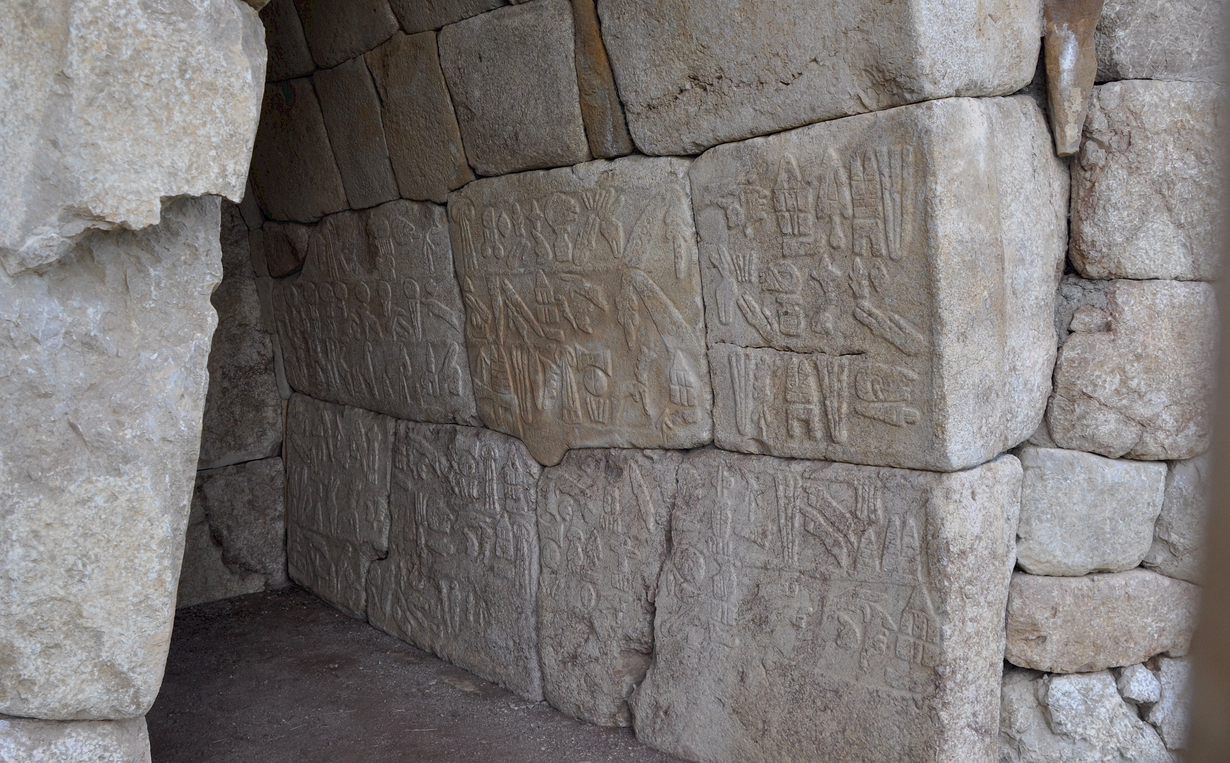
\includegraphics[width=\textwidth]{../../Mídia/BOGAZKOY_21.jpg}
		\caption{Inscrição BOĞAZKÖY 21. Dentro do complexo das piscinas sagradas de
			Hattusa, contendo o nome de Suppiluliuma II.\@ Imagens de
			\href{https://www.hittitemonuments.com/bogazkoy/}{Hittite
				Monuments}. Ver~\citet[p. 48ff.]{CHLI3}
		}\label{fig:bogazkoy21}
	\end{center}
\end{figure}

\begin{figure}[htb]
	\begin{center}
		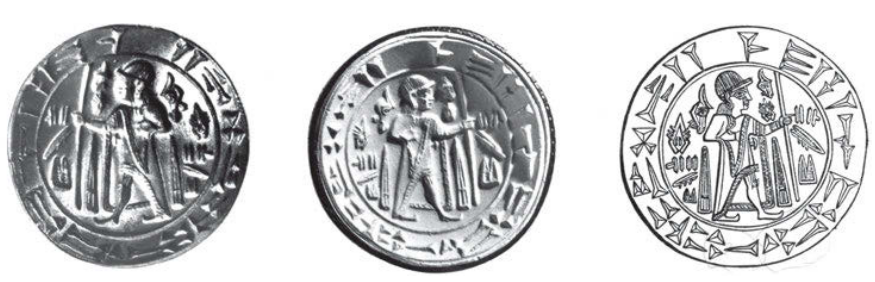
\includegraphics[width=\textwidth]{../../Mídia/tarkondemos.png}
	\end{center}
	\caption{Selo de ``Tarkondemos''. Digráfico com cuneiforme na circunferência e
		hieróglifos no centro. Atualmente o texto é interpretado como pertencente a
		um certo \emph{Tarkas{(sa)}nawa}. Final do século \textsc{xii aec}.
		Atualmente em Walters Art Gallery, Baltimore, no. 57.1512.
		Imagem e traçado de~\citet[p. 45f.; \emph{plate} 32]{CHLI3}
	}\label{fig:tarkondemos}
\end{figure}

\begin{figure}[htb]
	\begin{center}
		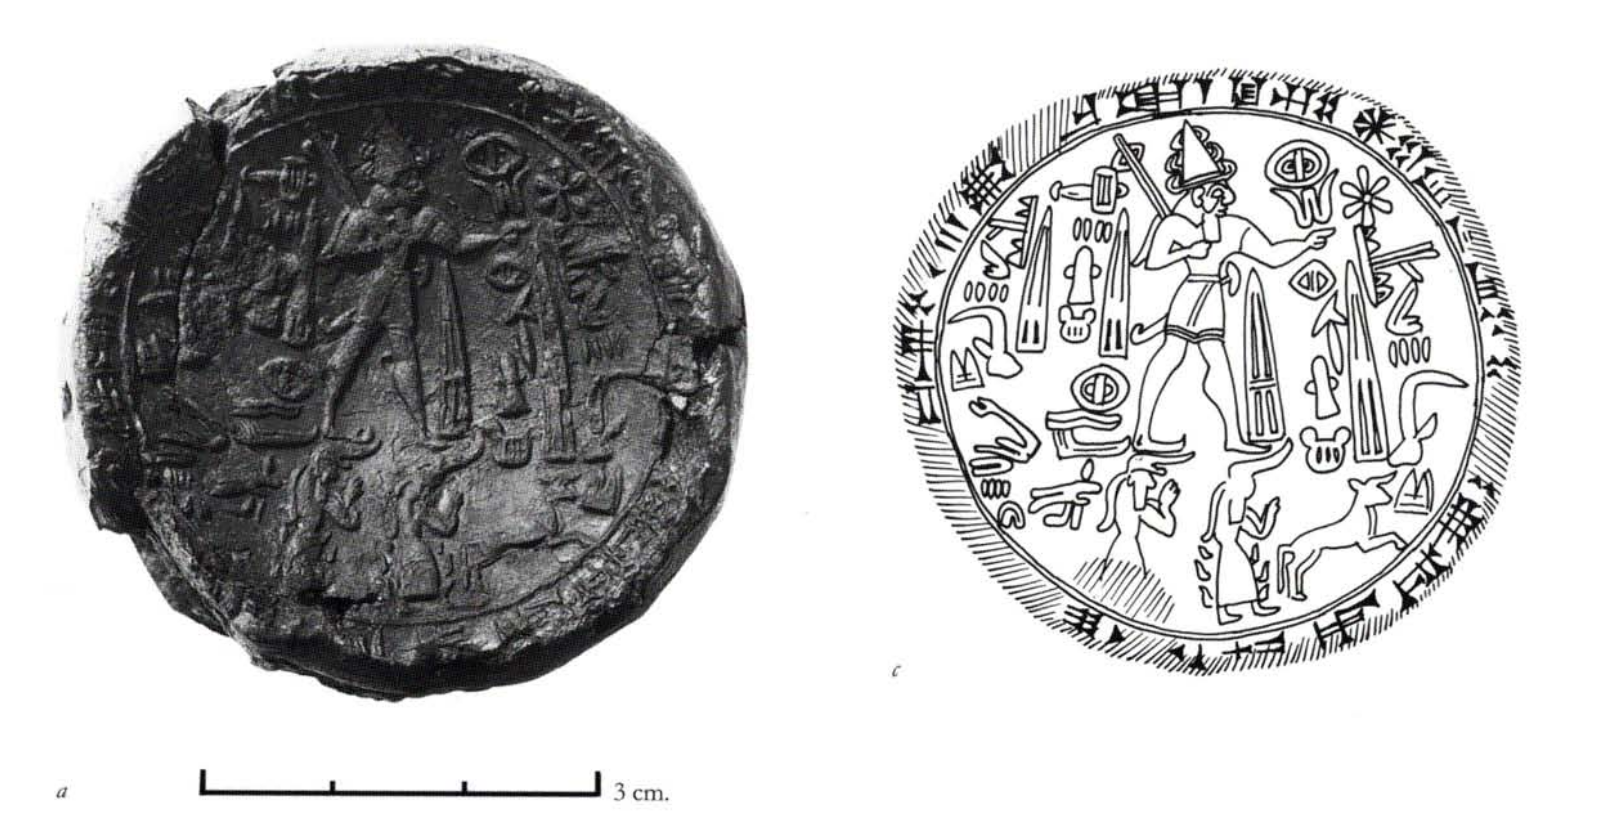
\includegraphics[width=\textwidth]{../../Mídia/lidar1.png}
	\end{center}
	\caption{Bula de LİDAR.\@ 5.4cm de diâmetro. Aproximadamente 1200 \textsc{aec}.
		Atribuído a Kuzi-Tešub, rei de Carquemis.
		Atualmente no Şanlıurfa Arkeoloji Müzesi.
		Imagem e traçado de~\citet[\emph{plate} 328]{CHLI13}}\label{fig:lidar1}
\end{figure}
\begin{figure}[htb]
	\begin{center}
		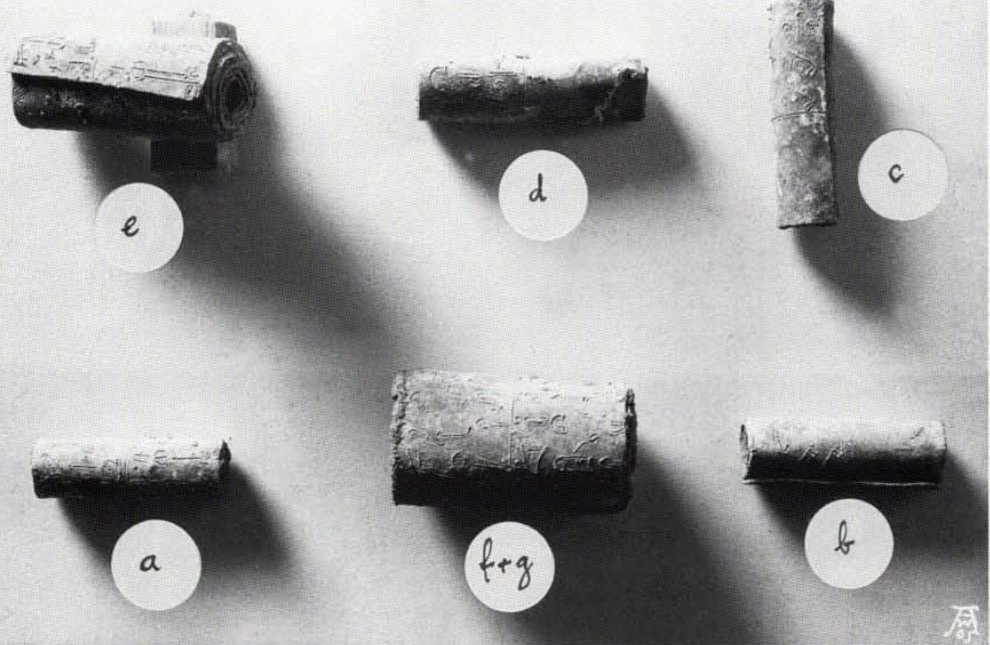
\includegraphics[width=\textwidth]{../../Mídia/assur1.png}
	\end{center}
	\caption{Cartas de Assur. Rolos de chumbo de aproximadamente 4cm de altura e
		diversas larguras contendo cartas de comerciantes.
		Escavados em Assur em 1905 pela Deutsche Orientgesellschaft.
		Originalmente alocados no Eski Şark Eserleri Müzesi, apenas os
		fragmentos \emph{e} e \emph{f} estão preservados e locados no
		Vorderasiatisches Museum, Berlin, no. VA 5819.
		Imagem de~\citet[\emph{plate} 306]{CHLI13}
	}\label{fig:assur1}
\end{figure}

\begin{figure}[ht!]
	\begin{center}
		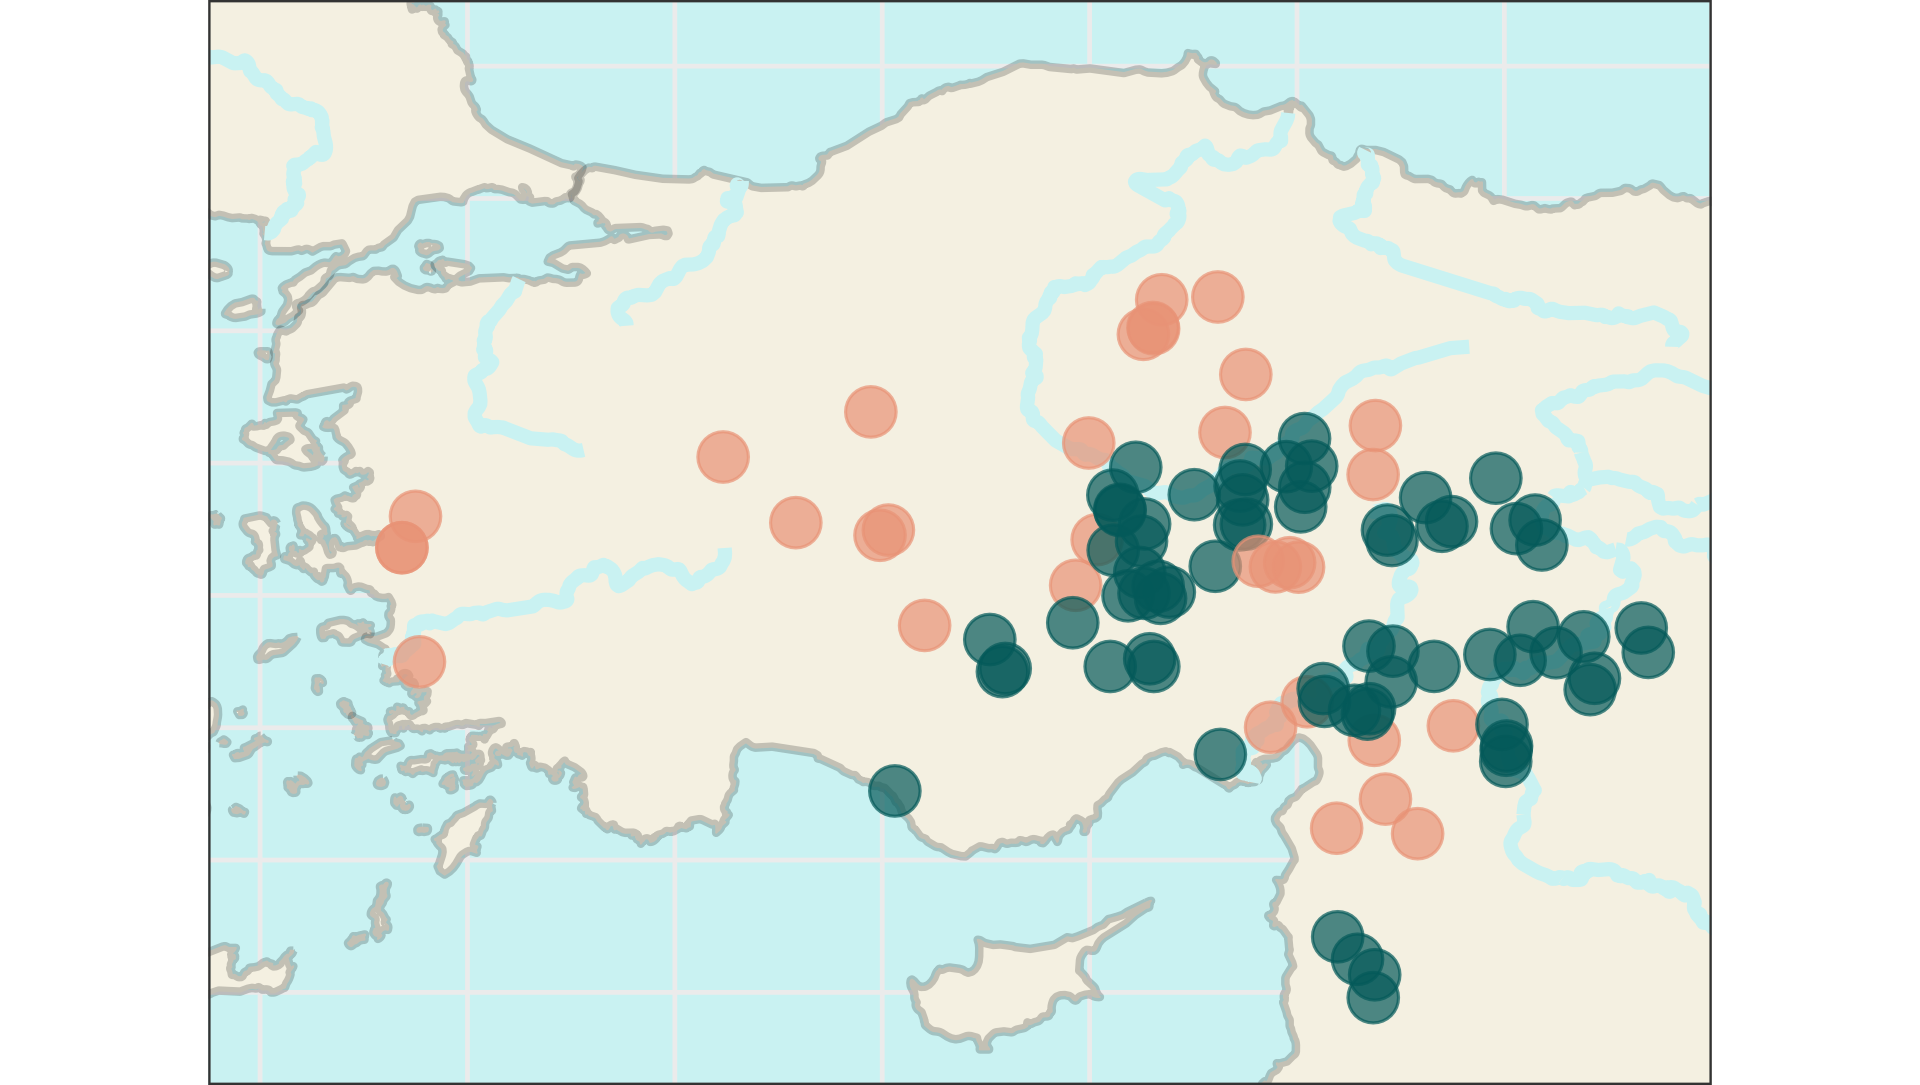
\includegraphics[width=1\textwidth]{../../Mídia/Map01.png}
	\end{center}
	\caption{Mapa contendo a localização das inscrições monumentais em luvita
		hieroglífico. Os pontos laranjas representam inscrições do período imperial
		enquanto os verdes, inscrições do período neo-hitita.}\label{fig:mapa1}
\end{figure}

\begin{figure}[ht!]
	\begin{center}
		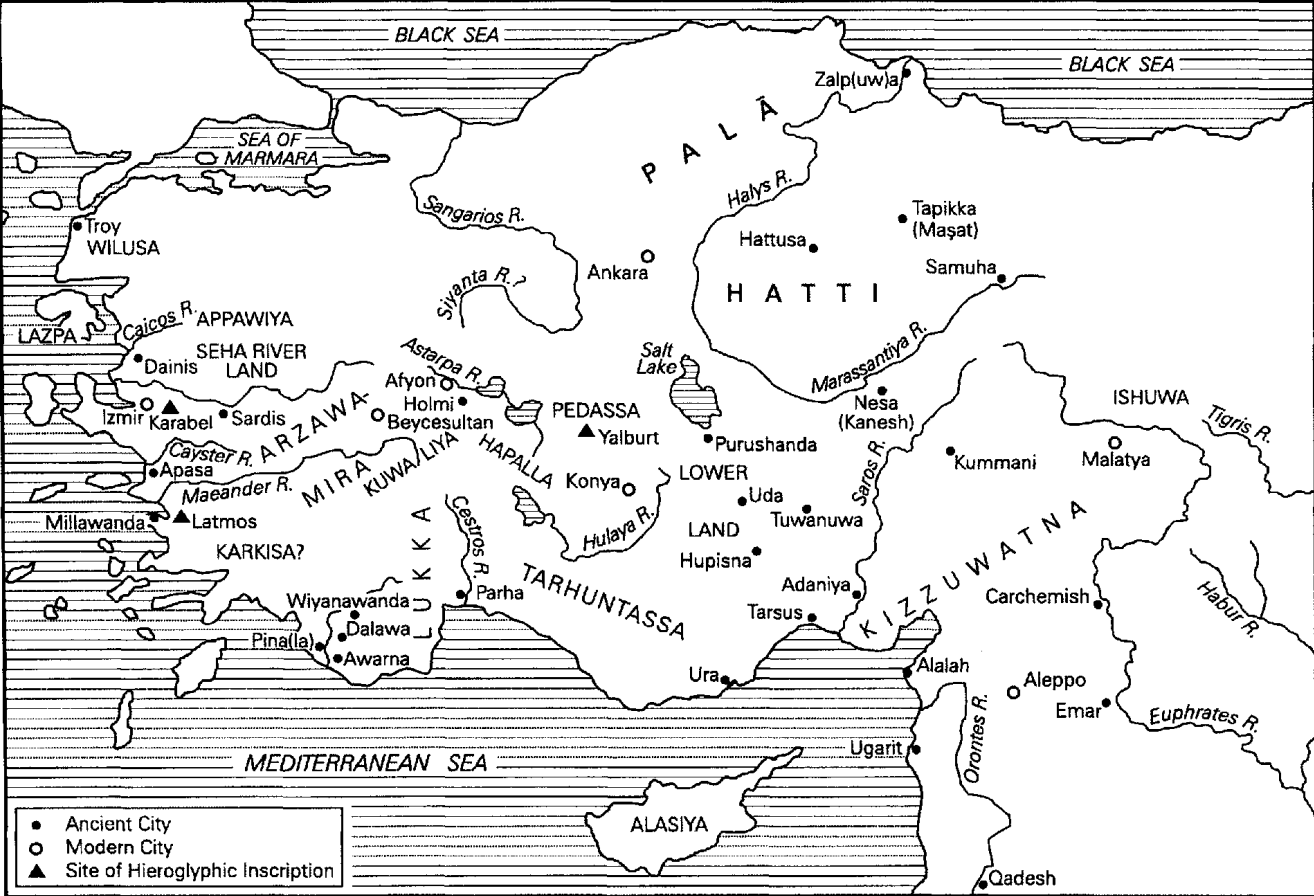
\includegraphics[width=0.95\textwidth]{../../Mídia/Mapa02.png}
	\end{center}
	\caption{Mapa da Anatólia durante a idade do bronze.
		\citet[37]{Melchert2003}.}\label{fig:mapa2}
\end{figure}

\vfill
\clearpage

\begin{figure}[!ht]
	\begin{center}
		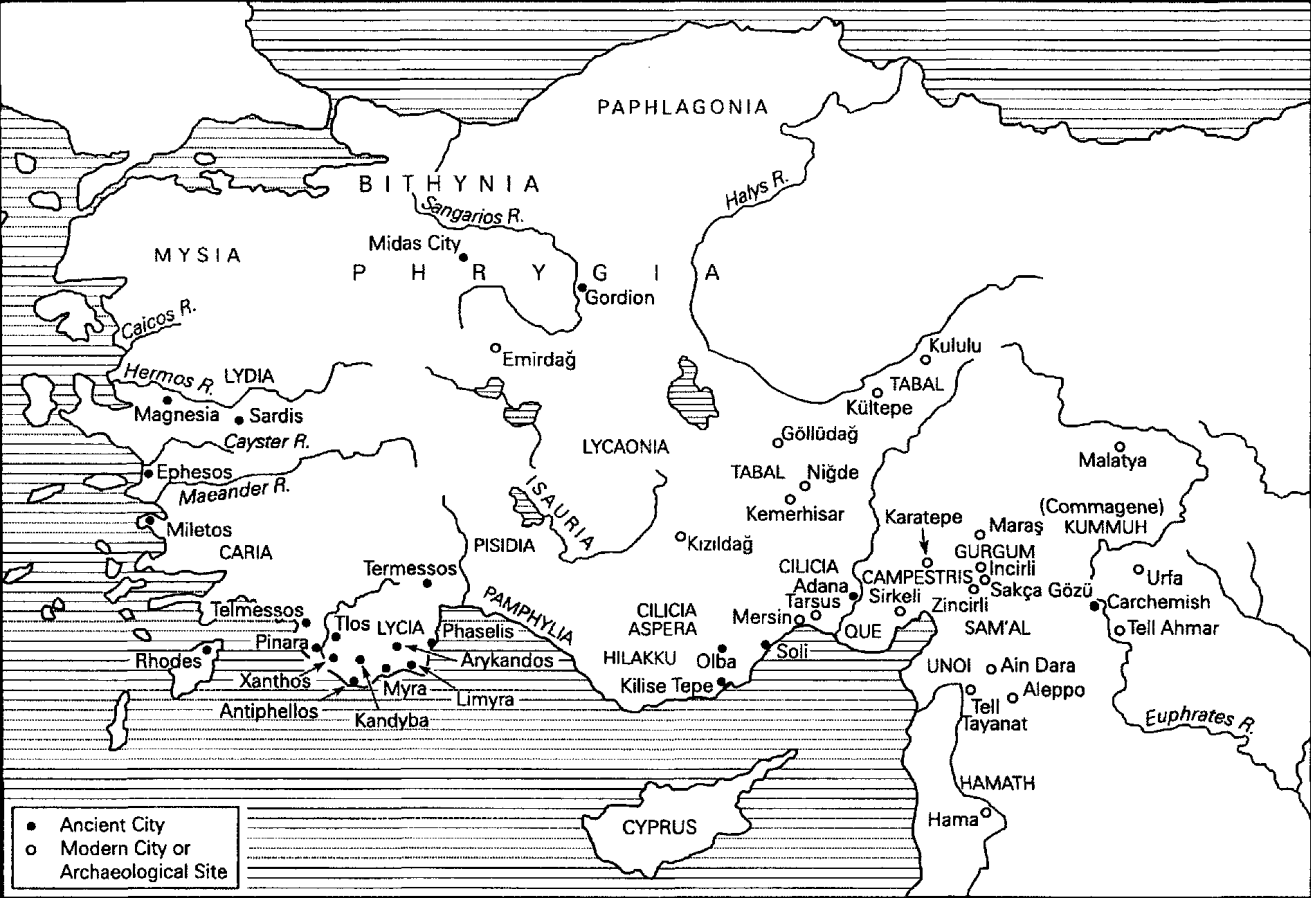
\includegraphics[width=0.95\textwidth]{../../Mídia/Mapa03.png}
	\end{center}
	\caption{Mapa da Anatólia durante a idade do ferro.
		\citet[94]{Melchert2003}.}\label{fig:mapa3}
\end{figure}
\vfill
